\chapter{Results and Discussion}
\label{chapterlabel4}
    \section{Parameters}
        \subsection{Flows}

        As evident from the observed movement patterns from the Mobility Dataset in Figure \ref{fig: observedflows_overview} , work-related and non-work-related flows exhibit a concentration of commuting trajectories within central London. Moreover, substantial flows are concentrated in the northeastern and southwestern regions of the city. The most notable difference between these two categories of flows lies in the concentration level: Work-related flows demonstrate a heightened level of convergence, whereas non-work-related flows display a distribution that extends spatially across a broader area.

    \begin{figure}[H]
        \centering
        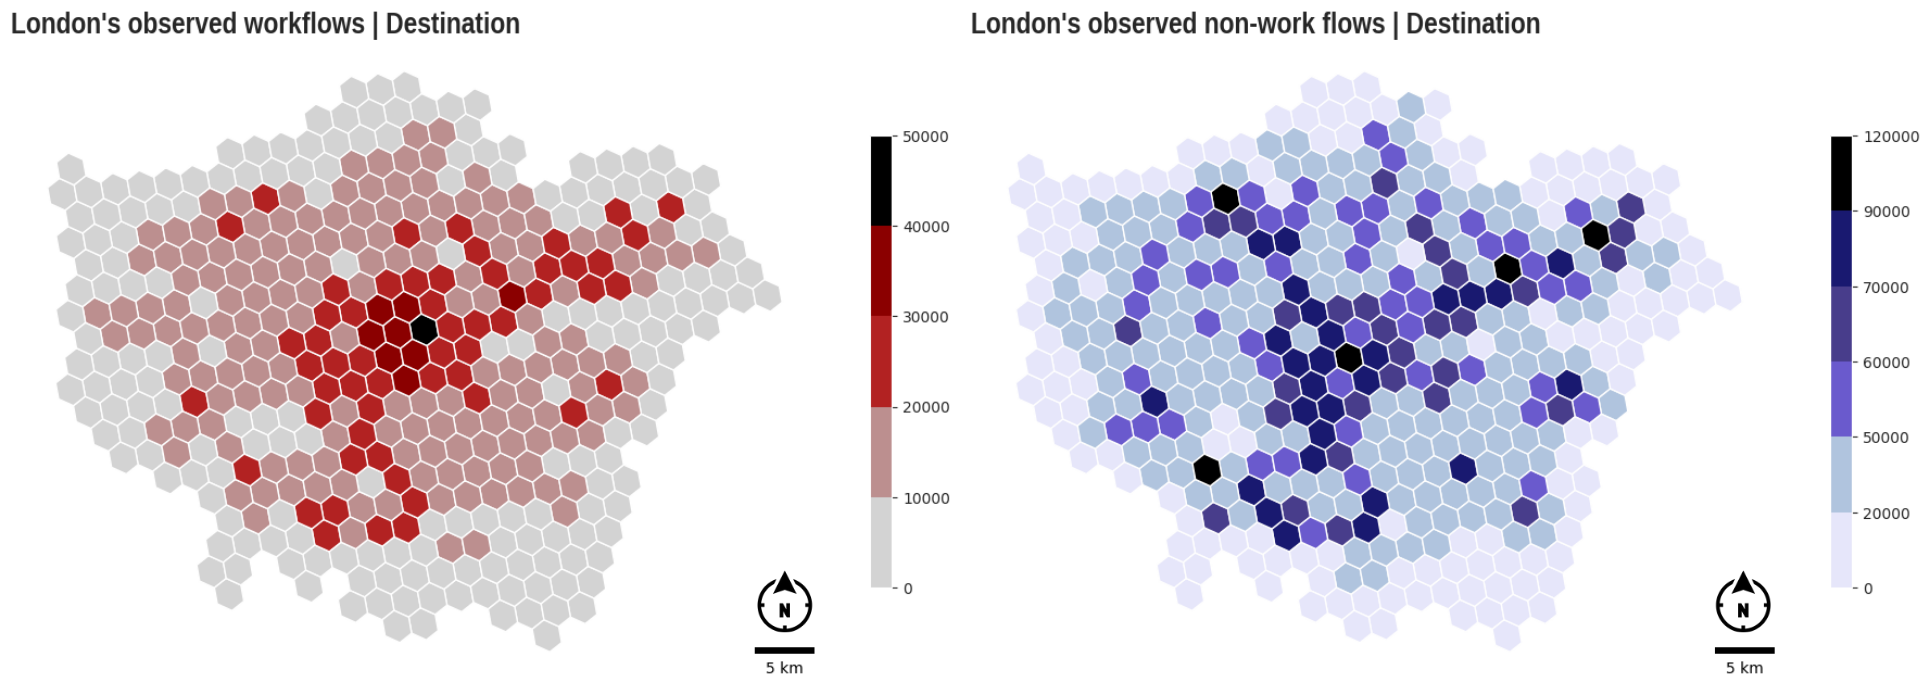
\includegraphics[width=15cm]{Images/Hex_observed_overview.png}
        \caption{London's observed flows: work and non-work.}
        \label{fig: observedflows_overview}
    \end{figure}

        \subsection{Features}


        

        \subsection{Attractiveness Factor}
        
        In the workflow regression analysis(Table \ref{tab:ols-results}), it is evident that the variables "EH," "PI," and "TR" have statistical significance since their p-values are low (all below 0.001). This indicates that these variables noticeably affect the dependent variable we are studying. Additionally, the high R-squared and adjusted R-squared values (0.863 and 0.860) signify that the model effectively explains much of the variation in the dependent variable.

        As part of the analytical refinement process, it was excluded the variables "CS" (commercial services) and "SE" (Sport and Entertainment). These variables were omitted due to their elevated p-values, above 0.4, signalling a lack of statistical significance. Additionally, both models exhibited a notably high condition number. However, a significant improvement was observed upon removing these two variables. The condition number, originally at 1.27e+03, was substantially reduced to a more manageable 647 in both regression models. 

\begin{table}[H]
\centering
\begin{tabular}{@{}lllll@{}}
\toprule
\textbf{Variables} & \textbf{coef} & \textbf{std err} & \textbf{P>|t|} \\ \midrule
Intercept & 932.6236 & 284.803 & 0.001 \\
AED & -14.0624 & 3.827 & 0.000 \\
AT & -42.8778 & 9.624 & 0.000 \\
\color[HTML]{9A0000} \textbf{EH} & \color[HTML]{9A0000} \textbf{33.2344} & \color[HTML]{9A0000} \textbf{6.902} & \color[HTML]{9A0000} \textbf{0.000} \\
MP & -32.6702 & 6.067 & 0.000 \\
\color[HTML]{9A0000} \textbf{PI} & \color[HTML]{9A0000} \textbf{80.2838} & \color[HTML]{9A0000} \textbf{6.608} & \color[HTML]{9A0000} \textbf{0.000} \\
RT & 5.8310 & 2.613 & 0.026 \\
\color[HTML]{9A0000} \textbf{TR} & \color[HTML]{9A0000} \textbf{18.1677} & \color[HTML]{9A0000} \textbf{6.916} & \color[HTML]{9A0000} \textbf{0.009} \\ \bottomrule
\textbf{R-squared} & 0.863 \\
\textbf{Adj. R-squared} & 0.860 \\
\textbf{Cond. No.} & 647. \\ \bottomrule
\hline
\end{tabular}
\caption{OLS Regression Results}
\label{tab:ols-results}
\end{table}

        Thus, within the context of workflows, the collective counts of Points of Interest from these three categories, namely "EH," "PI," and "TR," represent the Work-related Points of Interest. As shown in Figure \ref{fig: Regression_work}, these variables represent a linear relationship with the observed flows.

        \begin{figure}[H]
            \centering
            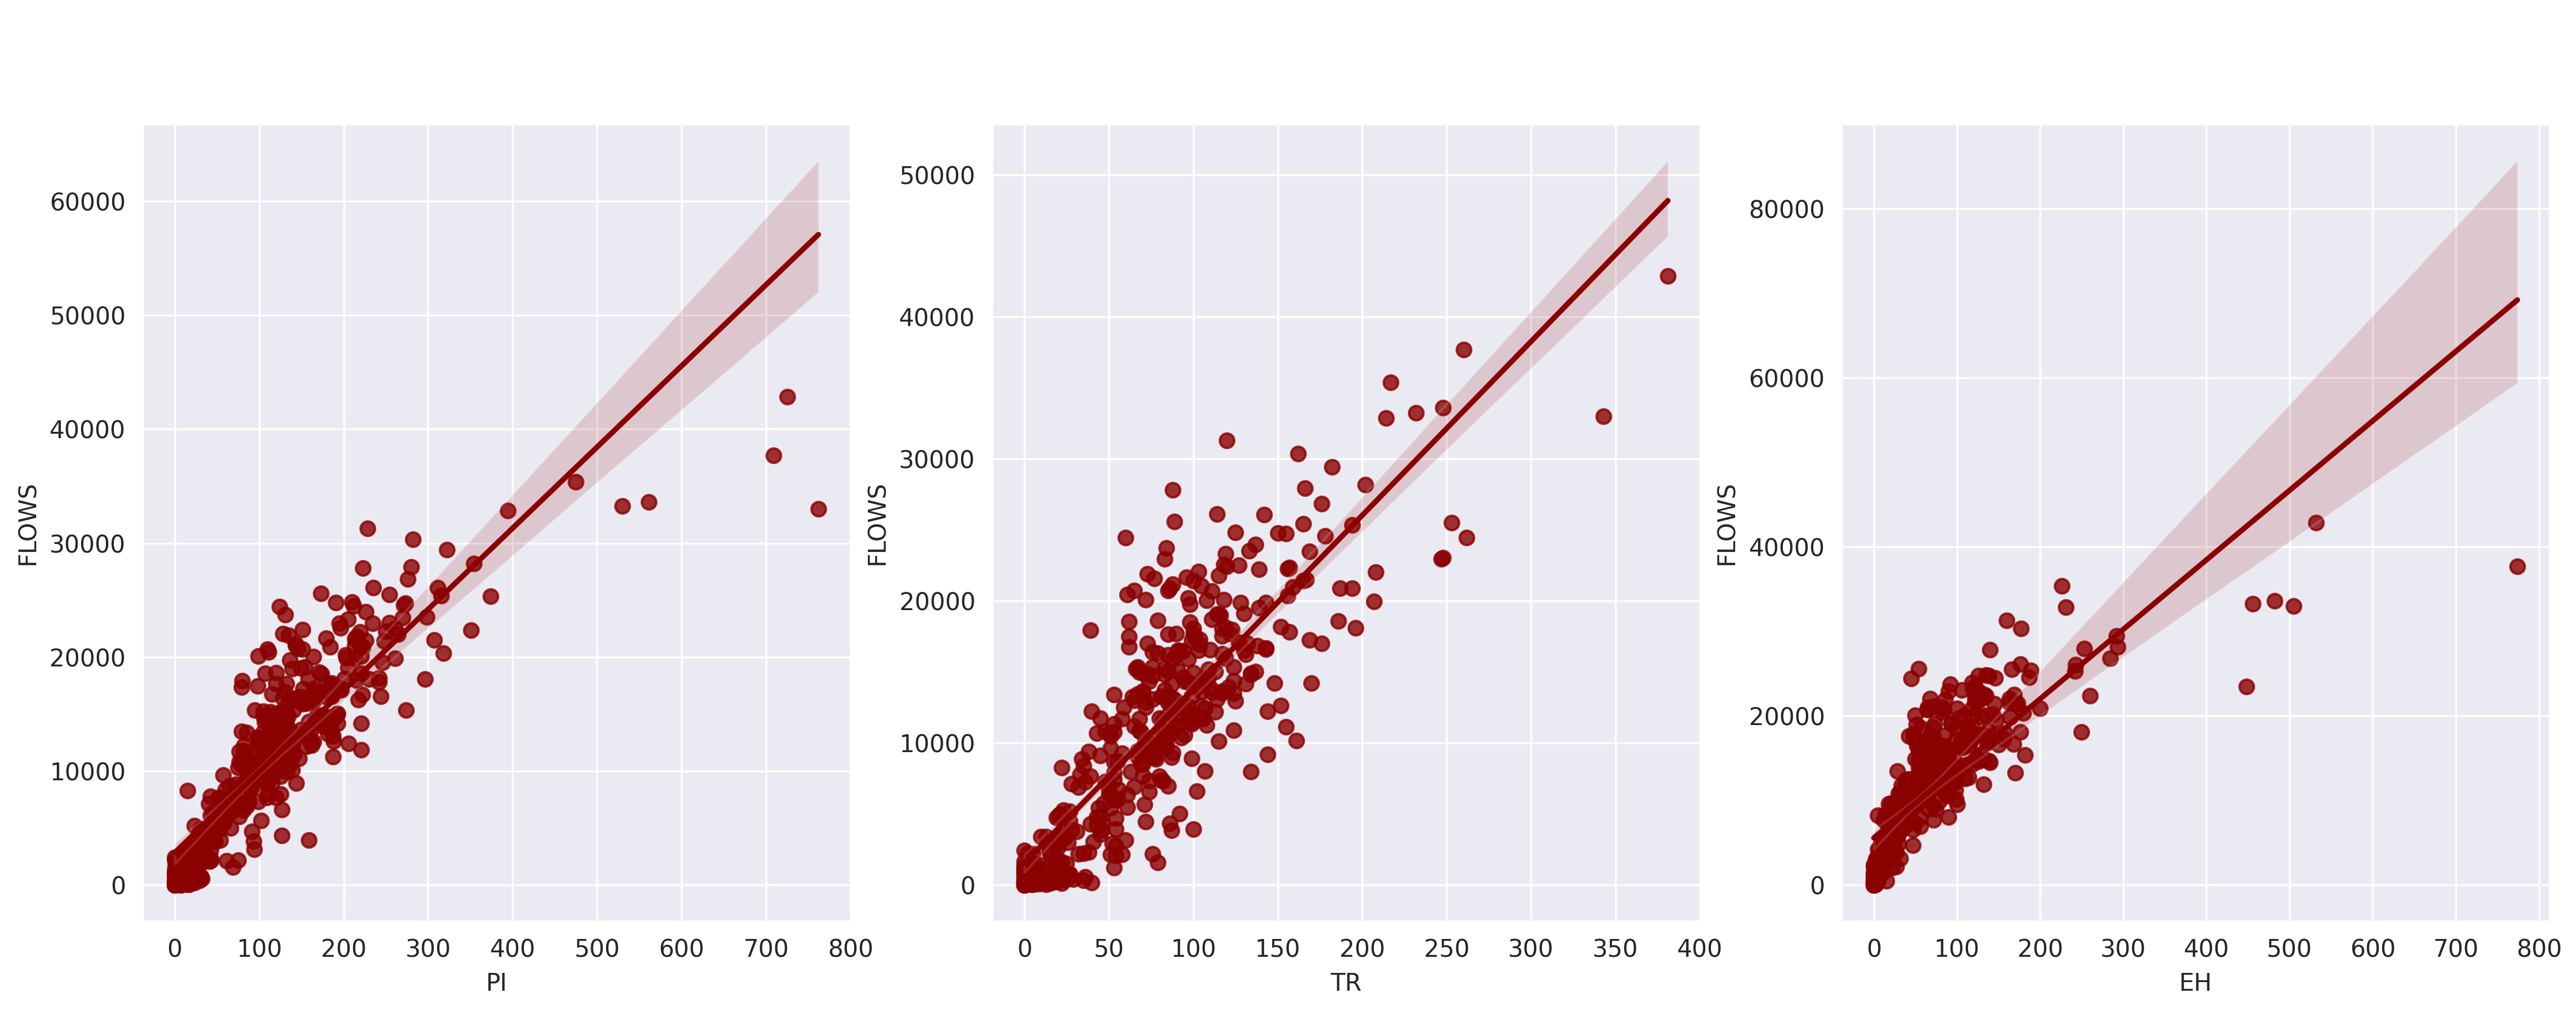
\includegraphics[width=14cm]{Images/regression_work.png}
            \caption{Work - Linear Regression: Flows vs POI}
            \label{fig: Regression_work}
        \end{figure}

        Regarding the non-work flows regression analysis in Table \ref{tab:ols-results-new-bold-color}, we observe that the variables "EH," "PI," "RT," and "TR" also demonstrate statistical significance, as their p-values are very low (all below 0.001). This implies that these variables significantly impact the dependent variable. The R-squared and adjusted R-squared values (0.782 and 0.778) indicate that our model effectively clarifies a significant portion of the variation in the dependent variable.  

        \begin{table}[H]
        \centering
        \begin{tabular}{@{}lllll@{}}
        \toprule
        \textbf{Variables} & \textbf{coef} & \textbf{std err} & \textbf{P>|t|} \\ \midrule
        Intercept & 5655.2406 & 1030.797 & 0.000 \\
        AED & -75.1430 & 13.851 & 0.000 \\
        AT & -201.4072 & 34.834 & 0.000 \\
        \textcolor{customblue}{\textbf{EH}} & \textcolor{customblue}{\textbf{113.3599}} & \textcolor{customblue}{\textbf{24.982}} & \textcolor{customblue}{\textbf{0.000}} \\
        MP & -131.6164 & 21.959 & 0.000 \\
        \textcolor{customblue}{\textbf{PI}} & \textcolor{customblue}{\textbf{218.6156}} & \textcolor{customblue}{\textbf{23.916}} & \textcolor{customblue}{\textbf{0.000}} \\
        \textcolor{customblue}{\textbf{RT}} & \textcolor{customblue}{\textbf{58.1842}} & \textcolor{customblue}{\textbf{9.456}} & \textcolor{customblue}{\textbf{0.000}} \\
        \textcolor{customblue}{\textbf{TR}} & \textcolor{customblue}{\textbf{73.5557}} & \textcolor{customblue}{\textbf{25.033}} & \textcolor{customblue}{\textbf{0.003}} \\ \bottomrule
        \textbf{R-squared} & 0.782 \\
        \textbf{Adj. R-squared} & 0.778 \\
        \textbf{Cond. No.} & 647. \\ \bottomrule
        \hline
        \end{tabular}
        \caption{OLS Regression Results}
        \label{tab:ols-results-new-bold-color}
        \end{table}

        In the non-work flows context, the combined counts of Points of Interest from these four categories, "EH," "PI," "RT," and "TR," symbolise the Non-Work-related Points of Interest. Thus, both regression models(Figure \ref{fig: Regression_nonwork}) appear well-suited for explaining the relationships between the independent and dependent variables.


        \begin{figure}[H]
            \centering
            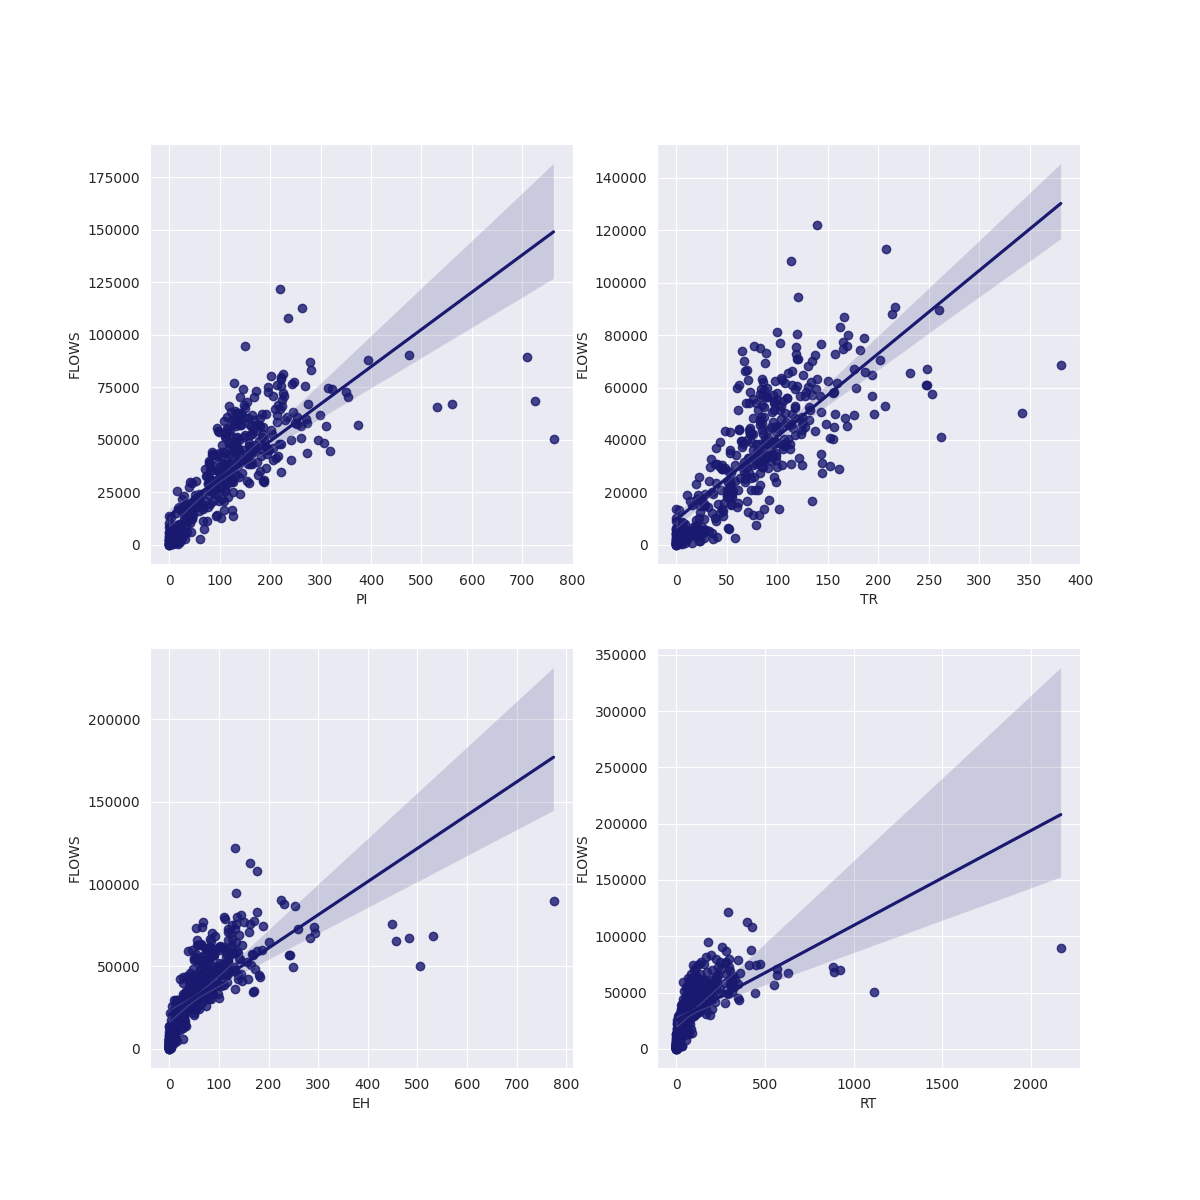
\includegraphics[width=14cm]{Images/regression_nonwork.png}
            \caption{Non-Work - Linear Regression: Flows vs POI}
            \label{fig: Regression_nonwork}
        \end{figure}


        In the context of residuals within both models(Figure \ref{fig: Residuals - Overview}), it is crucial to note that their distribution is normal, a fundamental assumption in regression analysis. This normal distribution holds significance because it indicates that errors in the model's predictions are distributed evenly around zero. Furthermore, the concentration of values is near zero when assessing the relationship between residuals and fitted values. This pattern confirms the suitability of the chosen linear regression models for the analysis.
        
        \begin{figure}[H]
            \centering
            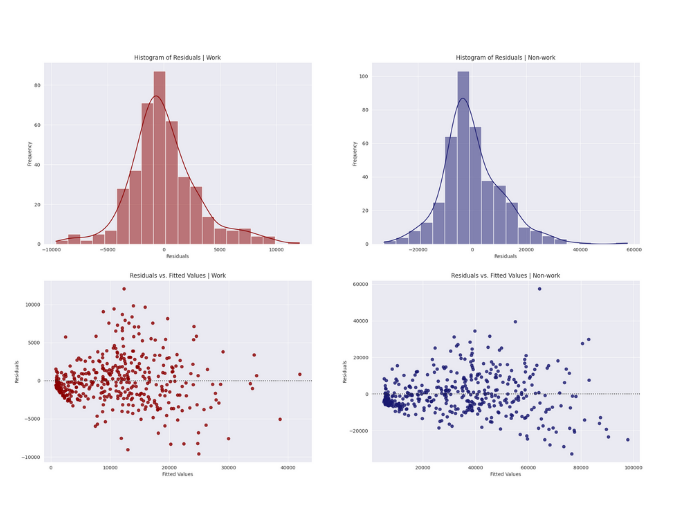
\includegraphics[width=14cm]{Images/Residuals_overview.png}
            \caption{Residuals - Overview}
            \label{fig: Residuals - Overview}
        \end{figure}
        
 

        The map below(Figure \ref{fig: POI_map}) illustrates the spatial distribution of Points of Interest (POI) in London, categorising them into work-related and non-work-related. It becomes evident that their distribution across the city exhibits a degree of similarity, predominantly concentrating in inner London instead of outer London. However, it is worth emphasising that the total number of points differs significantly due to the non-work category that contains four distinct POI groups. The POI values for non-work are also correlated with mobility flow values distribution, as the proportions remain consistent. Work-related flows represent only a fraction of the city's overall journeys, whereas non-work flows encompass a broader spectrum of activities.

        \begin{figure}[H]
            \centering
            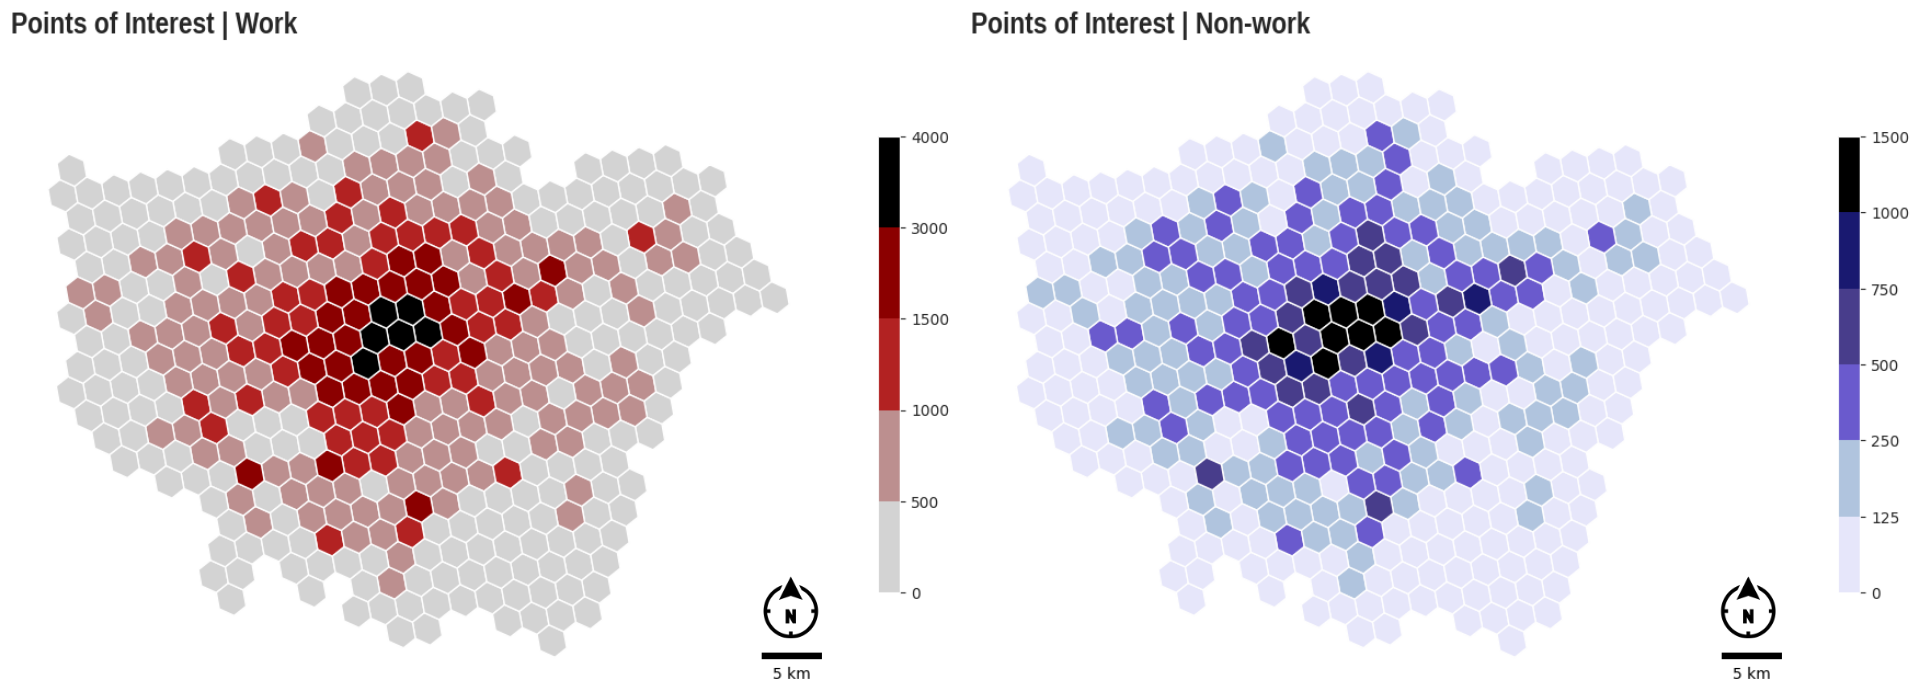
\includegraphics[width=14cm]{Images/POI_map.png}
            \caption{Points of Interest spatial distribution: Work and Non-work}
            \label{fig: POI_map}
        \end{figure}

        Additionally, the analysis reveals varying concentration patterns between the two categories of amenities. Work-related amenities exhibit a higher concentration in the city centre, whereas non-work amenities exhibit a more gradual and dispersed distribution throughout the city. This nuanced spatial distinction highlights these amenities' differential nature and accessibility for London's residents and visitors.

        \subsection{Population}
 
        To standardise the data, the 2021 census population data was aggregated, aligning it with the level 7 hexagons, as visually represented in the map below(Figure \ref{fig: Population Census}). This aggregation illustrate a significant concentration of residents within inner London, especially within the northeastern quadrant. While some other areas display a more dispersed spatial distribution, central London's concentration closely reflects the distribution patterns evident in the Points of Interest dataset and the mobility flows data.
        
        \begin{figure}[H]
            \centering
            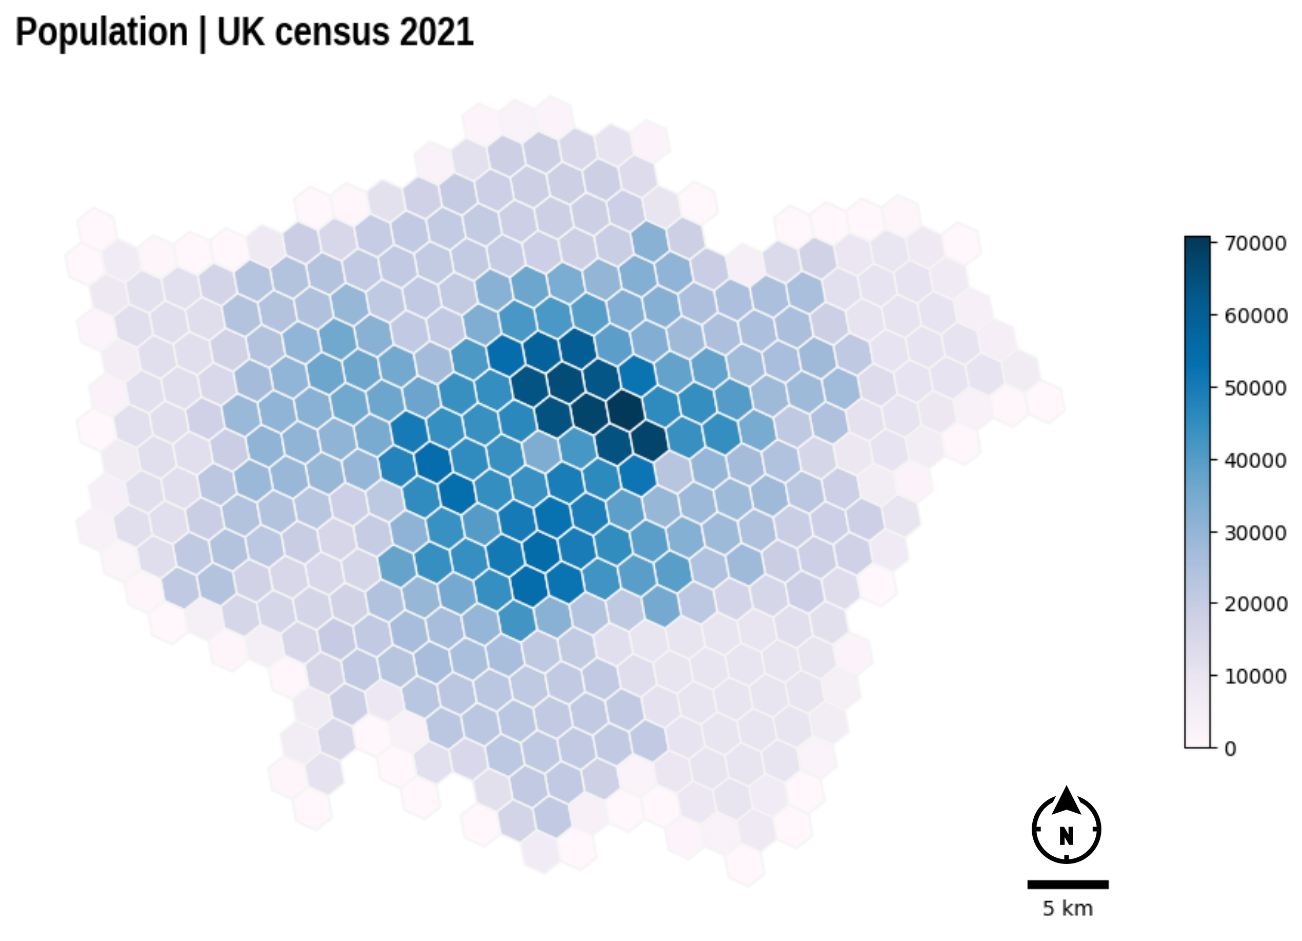
\includegraphics[width=12cm]{Images/population.png}
            \caption{Population - UK Census 2021}
            \label{fig: Population Census}
        \end{figure}
    
    \section{Analyzing the models comparatively}  

    The application of the spatial interaction model revealed limitations when processing the large dataset from the Mobility dataset. However, in contrast, the Deep Gravity Model demonstrated exceptional predictive capabilities, even in the face of substantial data volumes. The deep gravity model showcased its effectiveness when analyzing hexagons up to level 9, encompassing a vast geographical expanse of 17,636 hexagons and offering over 300 million potential origin-destination flows. On the other hand, the spatial interaction model was limited. It was restricted to operating exclusively within hexagons at level 7, where it relied upon the computational of a GPU equipped with high-performance RAM.

    The architecture of the Deep Gravity Model entails a division of geographic region units into distinct training and test groups, a feature that has contributed to its challenges in effectively managing Big Datasets. Consequently, the model generates results exclusively for the training sample. Therefore, to maintain the integrity and consistency in our comparative analysis across various models and flow types, we opted to employ the same sample for the Production-Constrained Model, aligning it with the dataset utilised for the Deep Gravity Model. This approach ensured a comprehensive and meaningful evaluation of model performance and the complex flow dynamics patterns aimed to uncover and understand.

    Some key findings in the regression plot(\ref{fig: Flows - Regression}) illustrate the relationship between the observed flows and those generated by the Deep Gravity Model (DG) and the Spatial Interaction Model (SIM). Therefore, the plot reveals a linear relationship on relationship between these variables. Furthermore, the graph unveils distinctive characteristics in the distribution of data values for each flow type. Specifically, when we examine the non-work flows, they exhibit a higher concentration, with values clustering closer to zero on the graph. In contrast, the non-work flows display a more dispersed pattern, with values distributed across a wider range of values. This divergence in the distribution patterns of the two flow types is a significant finding drawn from the regression plot. It emphasises the need for a differentiated analytical approach for each flow type.

            \begin{figure}[H]
            \centering
            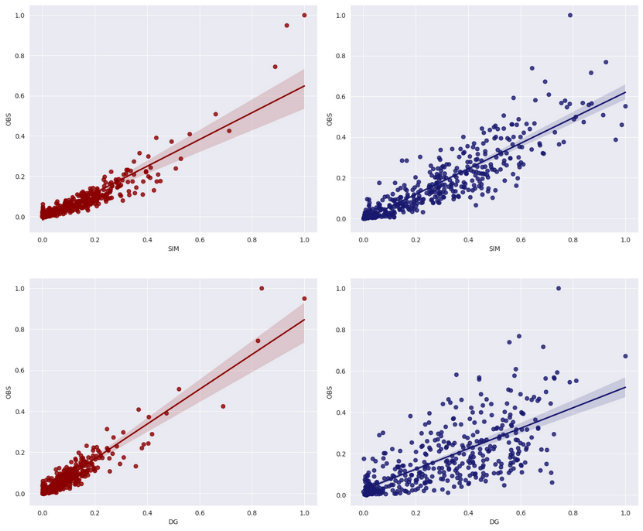
\includegraphics[width=14cm]{Images/Flows_regression.png}
            \caption{Flows - Regression plot}
            \label{fig: Flows - Regression}
            \footnotesize{\textbf{Red:} Workflows. \textbf{Blue:} Non-work flows.}
        \end{figure}

    In assessing the performance of the models in predicting flows, it is evident that the R-squared values for Non-work flows outperform those for workflows, with a notable high value of 0.7 observed in the production-constrained model for non-work flows and 0.9 in the Deep Gravity Model. In the context of workflows, the DG model achieved a better performance of 0.9, while the SIM model had 0.6.
    
    R-squared serves as a valuable metric for comprehending the influence of variables on flow prediction. Consequently, it becomes crucial to measure the efficacy of each model in estimating flows and the capability of selected independent variables in predicting the outcome. Among these variables, including distance, population, and the attractiveness factor derived from Points of Interest (POI), it is evident that they demonstrate superior performance in estimating flows, particularly within the Deep gravity model, outperforming the SIM model. Because of that, evaluating the Root Mean Square Error (RMSE) arises as an essential measure for comparing and evaluating the models against each other.

    The performance of the models displayed significant variations depending on the specific type of flow under consideration. It is important to highlight that the Production-Constrained Model, when put to the test, yielded the lowest RMSE value, achieving a relevant score of 14.69 for work-related flows. On the other hand, the Deep Gravity Model showcased a significantly lower RMSE value as well, standing at 41.47 for workflows. The model performance across these different flow types is concisely summarised in Table \ref{table: RMSE}, providing a comprehensive overview of how each model excelled in distinct aspects of mobility prediction.

            \begin{table}[h]
        \centering
        \begin{tabular}{@{}lll@{}}
        \toprule
        \textbf{Flows type} & \textbf{Deep Gravity} & \textbf{Production-Constrained} \\ \midrule
        Work                & 41.47                & 14.69                          \\
        Non-work            & 336.71                 & 141.19                          \\ \bottomrule
        \end{tabular}
            \caption{RMSE}
            \label{table: RMSE}
        \end{table}
    
    The contrast in model performance reveals a pattern: Models rooted in deep learning structures outperform the production-constrained model when predicting workflows. This result is evidenced by the high r-squared values and low RMSE (Root Mean Square Error) associated with these models. On the other hand, the prediction of non-work flows reveals a more complex context characterised by non-linear trajectories within the urban environment. Thus, both models achieve high r-squared values, with the deep gravity model slightly edging ahead. However, the SIM model records a lower RMSE value than the deep gravity model in this context.

    Nevertheless,  despite the spatial interaction model's computational limitations, the deep gravity model performs better when handling larger datasets. This is exemplified in Table \ref{table: RMSE_DG}, where the model demonstrates an r-squared of 0.7, lower than what was achieved at level 7. However, it is worth noting that the deep gravity model yields a lower RMSE, specifically 28.01, higher than the corresponding figure for the SIM model. Therefore, when the model aggregates data, the DG model experiences a decrease in performance in terms of RMSE, indicating the specificities of model behaviour under varying data conditions.
        
        \begin{table}[H]
        \centering
        \begin{tabular}{@{}lll@{}}
        \toprule
        \textbf{Flows type} & \textbf{Level 8} & \textbf{Level 7} \\ \midrule
        Work                & 433.65                & 41.47                          \\
        Non-work            & 28.01                 & 336.71                          \\ \bottomrule
        \end{tabular}
            \caption{RMSE- Deep Gravity Model at Hexagons level 7 and 8}
            \label{table: RMSE_DG}
        \end{table}
    
    
    In this context, the non-work flows contain various activities and behaviours within a city, such as leisure, tourism, and social interactions. These activities tend to follow less predictable patterns, making them challenging to model accurately. However, with its inherent capacity to capture intricate relationships and dependencies within the data, the Deep Gravity Model excelled in this aspect. It showcased its ability to predict the diverse and sometimes complex mobility patterns associated with non-work-related activities, producing lower error rates.
    
    The traditional Spatial Interaction Model demonstrated its comparative advantage in estimating flows characterised by a more linear and structured relationship, primarily those about work-related activities. Workflows often follow established commuting routes and daily routines, resulting in more predictable mobility patterns. In these scenarios, the traditional model indicated greater accuracy in the workflow predictions. However, it obtained an RMSE rate for non-workflows.
        
    In addition to the previously mentioned metrics, a spatial analysis of how the two models reflect estimated flows is crucial. By using the Observed Flows (OBS) as a reference, we can better comprehend how these metrics evaluate the performance of both the Deep Gravity Model (DG) and the Spatial Interaction Model (SIM). Moreover, values were normalised to compare the models.

    Examining the workflows illustrated on the left in red(see Figure \ref{fig: nWF Model after calibration}), it becomes apparent that both models exhibit a similar pattern of flow concentration in central London. However, there is a significant distinction: the SIM model tends to overestimate some of the flows, with disparities varying from 0.15 to 0.30 compared to the Observed Flows. In contrast, the DG model's flow estimations closely align with the distribution of the Observed Flows, reinforcing the significance of its low RMSE value.
        
        \begin{figure}[H]
            \centering
            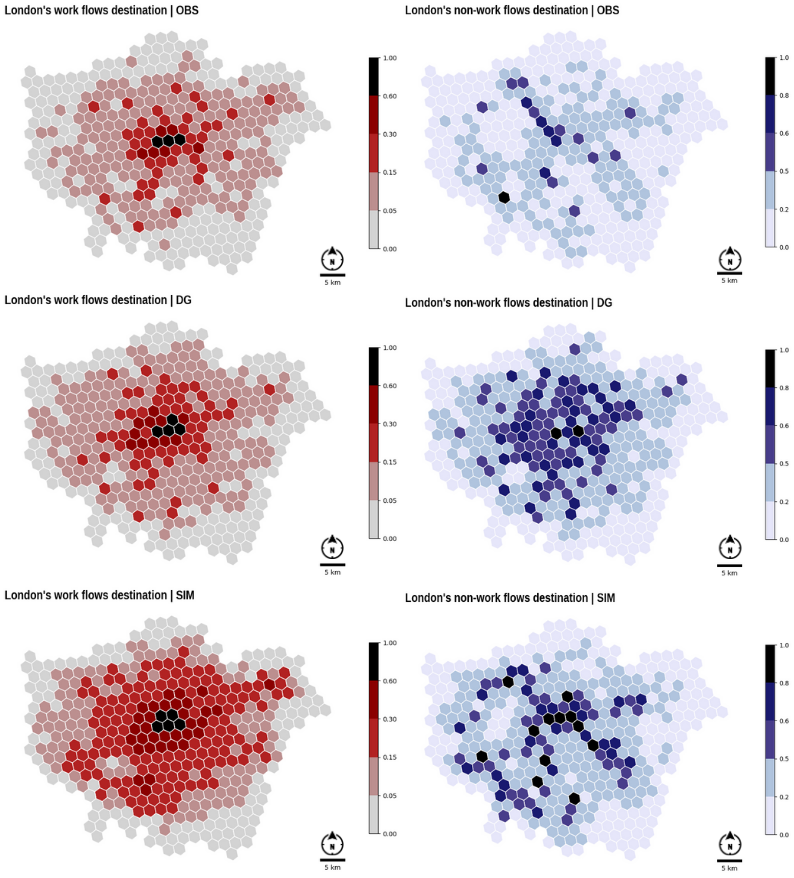
\includegraphics[width=15cm]{Images/Hex_comparativeanalysis.png}
            \caption{Observed and predicted flows for work and non-work flows}
            \footnotesize{OBS: Observed, DG: Deep Gravity, SIM: Spatial Interaction model, Red: workflows, Blue: non-workflows}
            \label{fig: nWF Model after calibration}
        \end{figure}

    Shifting our focus to the non-work flows shown on the right in blue, we observe a different outcome. At this level 7 of Uber hexagons, the Spatial Interaction Model displays greater accuracy in estimating non-work flow data, consistent with its previously noted low RMSE value. In contrast, the Deep Gravity Model tends to overestimate the flows, with disparities ranging between 0.5 and 0.6 compared to the Observed Flows. These spatial insights further illustrate both models' nuanced performance characteristics regarding their strengths and limitations in different flow scenarios.    

%%%%%%%%%%%%% DISCUSSION
        
\section{Discussion}

       The attractiveness factor utilised in the Spatial Interaction Model for Work and Non-work flows was constructed based on the categories within the POI dataset; see Figure \ref{fig: Attractiveness factor}. In the context of Workflows, the analysis revealed that Public Infrastructure (PI), Transport (TR), and Education and Health (EH) emerged as the most significant variables in the data collected from Mobility Data. In contrast, for the Non-work attractiveness factor, the primary variables align with those of the Workflows, except for Retail (RT).

        \begin{figure}[H]
            \centering
            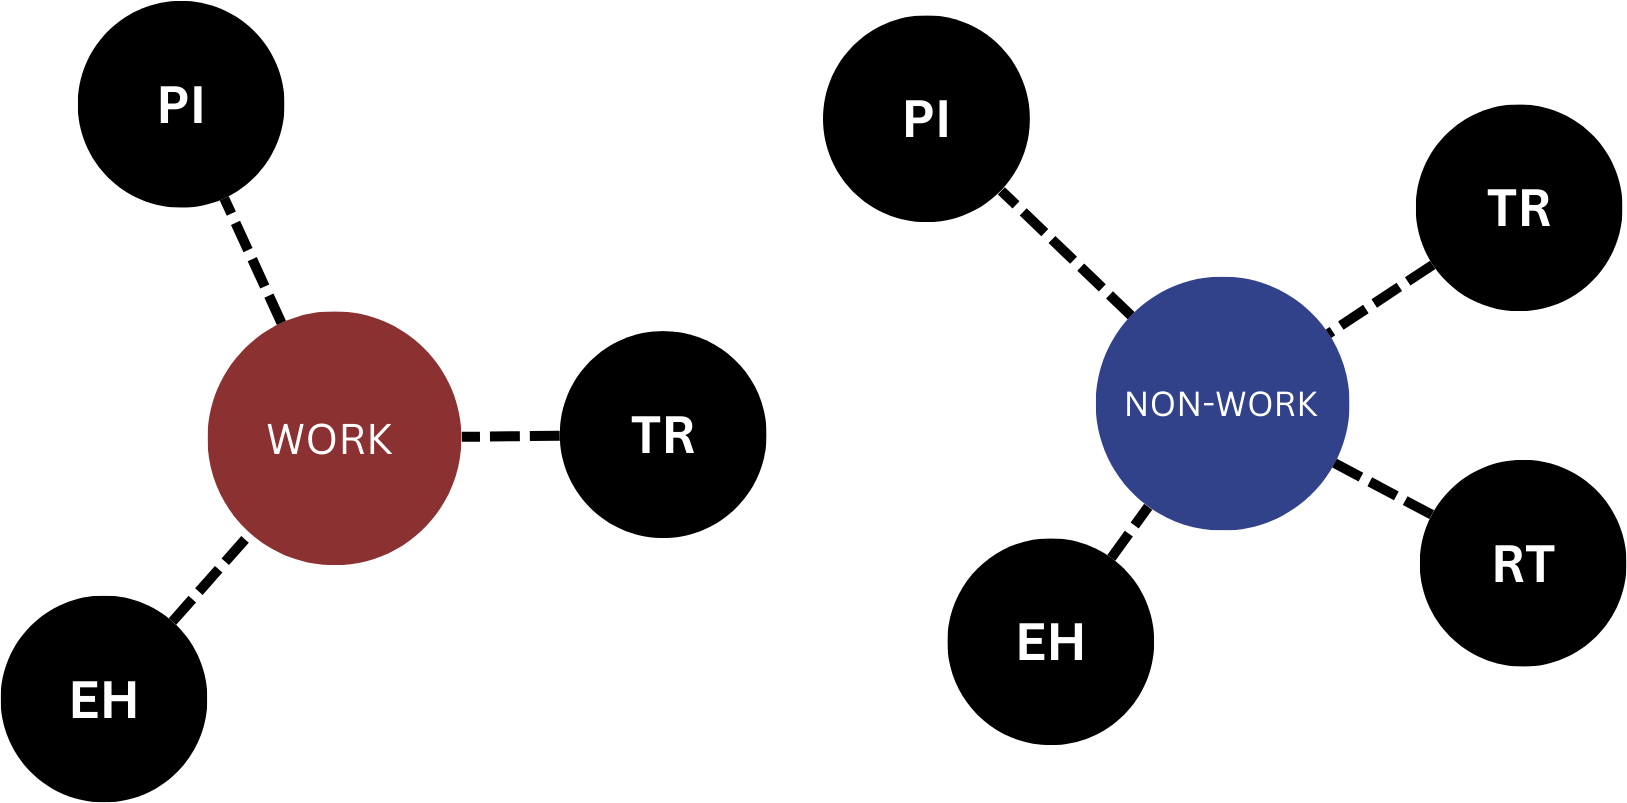
\includegraphics[width=14cm]{Images/Atractiveness factor.png}
            \caption{Attractiveness factor}
            \label{fig: Attractiveness factor}
        \end{figure}

       Mobility data sourced from Locomizer has emerged as a valuable and contemporary resource for analysing commuting dynamics. The data used in this study, collected in March, contrasts with the 2021 Census data on Origin and Destination. While both datasets primarily target the retail market, they offer profound insights into urban planning, which is increasingly influenced by dynamic factors. These factors encompass climate crises, ranging from intense rainfall to scorching heat waves and socioeconomic variables, exemplified by recent strikes in various sectors across England.

        Locomizer's dataset extends many possibilities for spatial analysis, many of which still need to be explored within the scope of this research. It offers the potential to unravel travel patterns by transportation mode and delve into user trajectories at different times of the day. Thus, it can provide hypotheses about how mobility impacts the city's dynamics across various temporal dimensions.

        Regarding the features considered, this analysis primarily focused on geographic data related to the Points of Interest dataset. However, given that the Deep Gravity Model can accommodate up to 18 features in its vector, integrating additional databases, such as OpenStreetMap, holds the promise of introducing greater complexity. This complexity would help characterise the geographic region under study, the mobility flows, and the factors influencing urban movement.

        Including the population census dataset played a pivotal role in running the four models. Nevertheless, it would be essential if Locomizer's Mobility data provided information on the Visitation Modality for worker users and residents. Despite indications in the dataset's documentation that such information is available, the version used for this research needed to have this important component. Including resident data could enhance data integrity and deepen our understanding of user mobility patterns within the Locomizer system.

        The impressive performance of the Deep Gravity Model when handling large datasets underscores the potential of new models that leverage machine learning techniques, including deep learning. The model's capability extends to analysing hexagons up to level 9, encompassing 17,636 hexagons and 300 million origin and destination possibilities. These models enable the effective management of complex, contemporary databases that demand enhanced computational capabilities. However, documentation is crucial for reproducible analysis, especially for the Deep Gravity model, which boasts a sophisticated and innovative structure for flow estimation. The lack of comprehensive documentation regarding input data structure and the complex code structure, employing PyTorch posed challenges when applying the large mobility dataset to the model.

        Both models demonstrated strong performance in estimating flows, yet the analysis context proved critical in determining the most suitable methodology. The SIM model excelled with aggregate data, while the Deep Gravity model performed better with granular data, even operating at the hexagon level 9 to estimate origin-destination flows. However, the results highlighted the ongoing complexity and challenges of estimating non-work-related flows. Even the Deep Gravity model, with its new structure and advanced computational methods, faced limitations in predicting these flows accurately.

        This outcome offers valuable insights into the relationship between these two flow types concerning user destinations. However, it is important to clarify that these Points of Interest do not necessarily imply exclusive representation of workplaces or leisure destinations. Instead, it signifies the coexistence of amenity categories within specific geographic regions (hexagons), where opportunities for work or leisure naturally converge.

        To illustrate further, in the context of workflows, the coexistence of Points of Interest related to Public Infrastructure, Transport, Education, and Health suggests a probable concentration of work-related activities within that region. Conversely, non-work flows, which include Retail as a significant variable, present intriguing complexities. These flows encompass activities unrelated to work, such as visits to parks, schools, and cafes. Consequently, the aggregation of these four amenity types closely reflects the destinations of individuals in London who are primarily there for non-work-related purposes, thereby enriching our understanding of the diverse dynamics of urban mobility.

        In this study, a series of critical questions deserve careful consideration:
        
        Firstly, evaluating the relative performance of the Deep Gravity Model in estimating carbon emissions within the London area is essential. This assessment provides valuable insights into the model's effectiveness in capturing the complex dynamics of carbon emissions, which is crucial for understanding urban environmental impact. Secondly, the combined analysis of the Deep Gravity Model with accessibility measures presents a crucial path for investigation. This integration can enhance the model's predictive capacity by leveraging accessibility data, providing a more comprehensive understanding of the factors influencing carbon emissions.
        
        Besides that, it is crucial to consider the limitations inherent in this analysis. Thus,  consider additional performance metrics that can comprehensively assess the Deep Gravity Model's effectiveness relative to alternative methodologies to ensure a robust comparison.This broader perspective facilitates a comprehensive understanding of the strengths and weaknesses of each model, leading to more informed conclusions regarding their respective capabilities in mobility flow estimation. 
        
        The primary concern is that the two primary metrics commonly utilised in this context, namely R2 and RMSE/SRMSE, have previously been indicated as inadequate representations of the actual inherent model performance due to the unique characteristics of spatial interaction flow. Consequently, this can result in erroneous deductions regarding relative performance (Knudsen \& Fotheringham, 1986) \cite{wilkinsonSpatialInteractionModels2023}. Despite the complexity of the datasets involved, particularly the Mobility Data, and the inclusion of multiple models (totalling four models), the principal focus of this study remains centred on utilising RMSE as the primary parameter and supplementing it with R-squared for individual model performance. However, it is crucial to acknowledge the limitation \cite{wilkinsonSpatialInteractionModels2023} outlined for a more comprehensive analysis. As emphasized by Wilkinson, when assessing the efficacy of spatial interaction models, it becomes crucial to account for the outcomes generated by these models, ensuring their alignment with the dataset. He warns against only using a single metric for evaluation, as such an approach might generate inaccurate conclusions regarding modelling performance. Thus, it resonates with the view that an evaluation is necessary to avoid misguided interpretations.
        
        Furthermore, \cite{wilkinsonSpatialInteractionModels2023, lucaSurveyDeepLearning2021} highlights a key consideration - the overall usage of two key metrics, R-squared and RMSE/SRMSE, may not necessarily capture the genuine underlying performance of a model. It is attributed to the inherent characteristics of spatial interaction flow, leading to potential inaccuracies in determining relative performance. Knudsen and Fotheringham (1986) suggest that these metrics might only partially reflect the true model performance due to the complex dynamics inherent in spatial interaction.  Combining these perspectives, it is evident that while RMSE and R-squared offer valuable insights, their limitations must be acknowledged. Particularly, the exclusion of additional evaluation criteria and the potential inadequacy of certain metrics in capturing complex spatial dynamics need to be recognised. Additionally, as \cite{wilkinsonSpatialInteractionModels2023} recommends, understanding how different features and datasets contribute to model performance is vital, especially in scenarios involving the integration of new datasets
        
        Lastly, the scope of this analysis is limited to a specific day of the year. A broader temporal evaluation, encompassing an extended period, would greatly contribute to understanding the model's performance over time, enabling insights into its stability and consistency across varying time frames.








